\documentclass[11pt]{article}
\usepackage{report}

\begin{document}
\section{The Fourier Transform of a Gaussian}
For this assignment we look at at the fast fourier transform of the Gaussian
\begin{equation}
	x(t) = \frac{1}{\sqrt{\pi \alpha^2}} e^{-t^2/\alpha^2}
	\label{eq:gaussian}
\end{equation}
and compare it with its true theoretical Fourier transform
\begin{equation}
	X(f) = e^{-\frac{1}{4} (2 \pi \alpha f)^2}.
	\label{eq:guassianFFT}
\end{equation}
\begin{figure}[H]
	\centering
	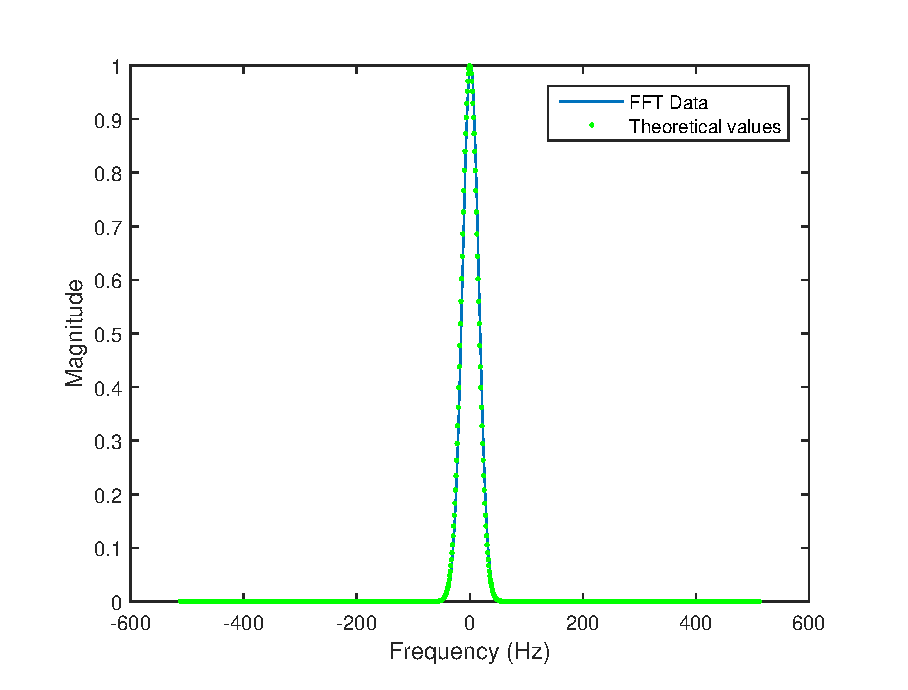
\includegraphics[width=1\textwidth]{../ex1/gaussianFFT}
	\caption{Comparison between the normalized fast fourier transform and the true theoretical fourier transform of the Gaussian (eq. \ref{eq:gaussian})}
	\label{fig:gaussianFFT}
\end{figure}

As we can see in figure \ref{fig:gaussianFFT} the fast fourier transform seem to be pretty spot on. The resolution of the frequencyis dependent on the sampling frequency and the amount of samples taken. This because the amount of samples taken directly translates on to haw many different frequency values we can get out of the transform\footnote{Due to the linearity of the transform we get one output for each input}. The sample frequency tells us which frequencies we could possibly have caught since one needs two points to capture a period. Basically we have frequencies in the range $[-\frac{1}{2 \Delta},\frac{1}{2 \Delta}]$, where $\Delta$ is the time between samples and since we simulate that we take 1024 samples we get 
\begin{align}
	&(\frac{1}{2 \Delta} +\frac{1}{2 \Delta})/\textit{number of jumps between frequency values} \\ 
	=& (\frac{1}{2\Delta} +\frac{1}{2\Delta})/1023\\
	=& 1024/1023 = 1.001.
\end{align}
This basically means we have 1.001 Hz between the frequencies we get checked in the fourier transform.

\section{The Fourier Transform of a Gaussian}
In this exercise we look at the equation 
\begin{equation}
	u(t) = \bar{u} sin(2 \pi f_c t )
\end{equation}
where $f_c = 8$ and $\bar{u}$ basically is a square wave going between the value 1 and a value $u_1$ which we vary through the exercise. The square wave changes values after a period of the sine function has passed. This is to simulate a message 01010101. Thus we plot the function for one whole time unit. 
\begin{figure}[H]
	\centering
	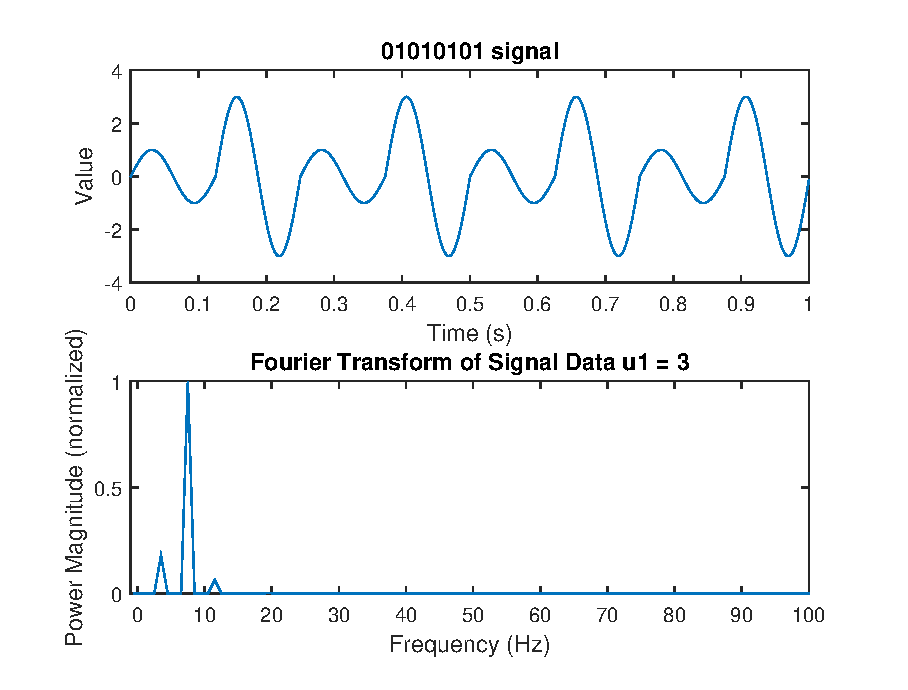
\includegraphics[width=1\textwidth]{../ex2/fftU1-3}
	\caption{Looking at the frequency spectrum of the signal with $u_1 = 3$.}
	\label{fig:fftU1-3}
\end{figure}
\begin{figure}[H]
	\centering
	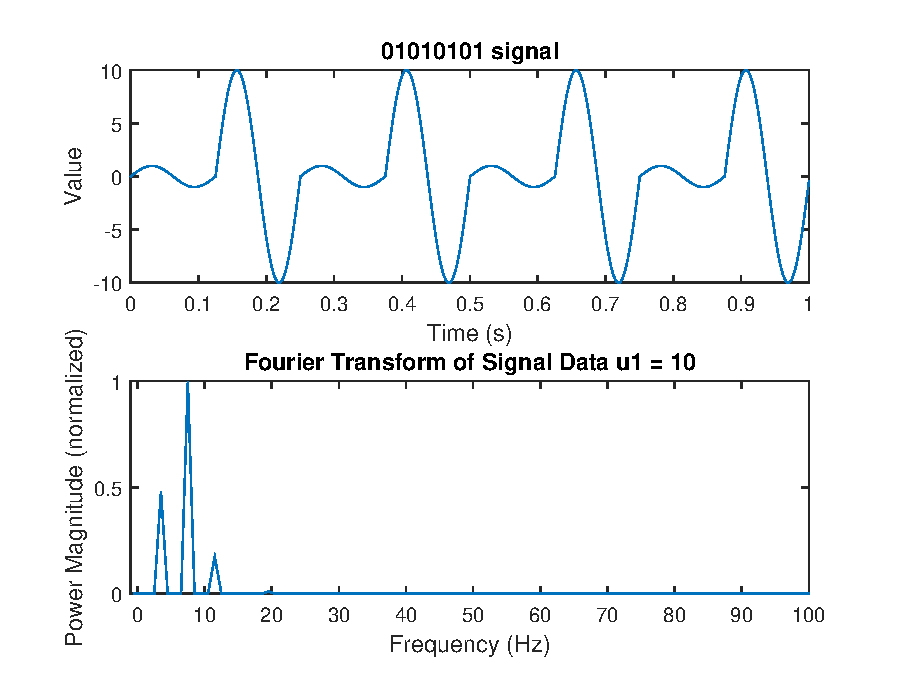
\includegraphics[width=1\textwidth]{../ex2/fftU1-10}
	\caption{Looking at the frequency spectrum of the signal with $u_1 = 10$.}
	\label{fig:fftU1-10}
\end{figure}

\begin{figure}[H]
	\centering
	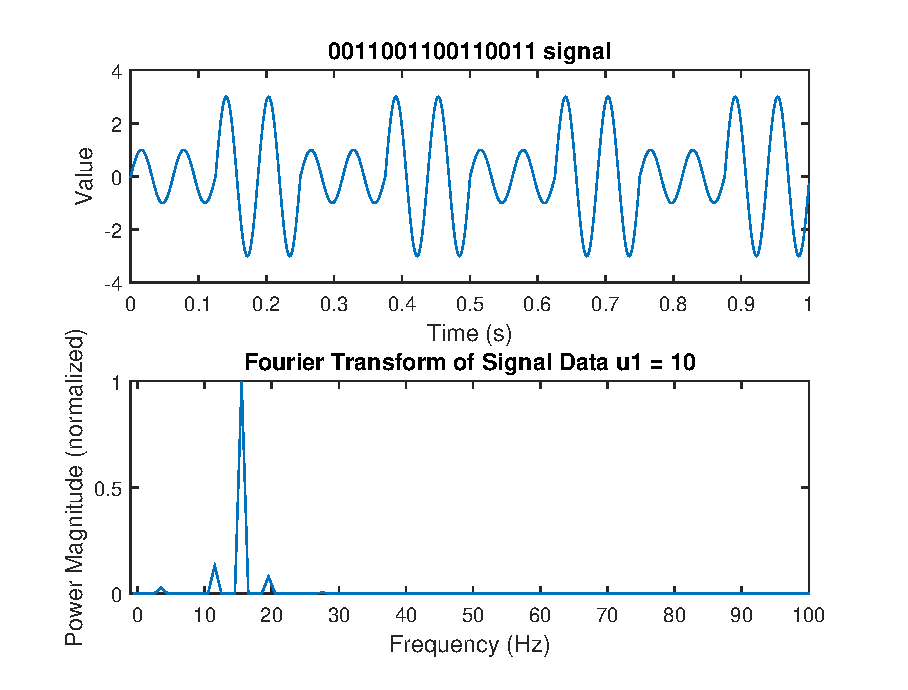
\includegraphics[width=1\textwidth]{../ex2/fftU1-3-double-same}
	\caption{Looking at the frequency spectrum of the signal with $u_1 = 3$. Ontop of that we doubled the carrier frequency without changing the modulation of the sine function. We can see that we have the same bandwidth but the same ammount of information is given.}
	\label{fig:fftU1-3}
\end{figure}
\begin{figure}[H]
	\centering
	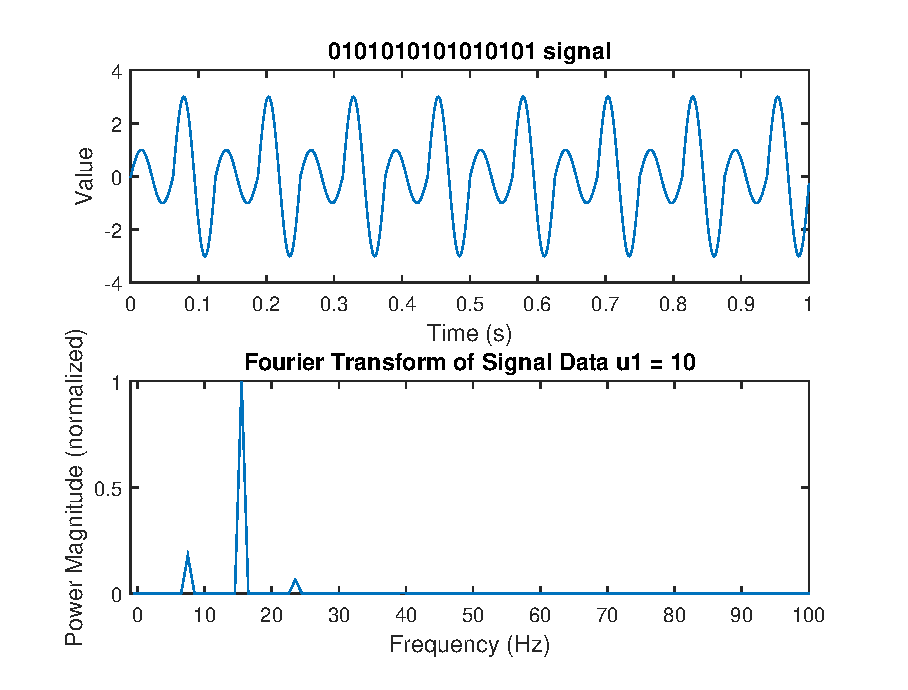
\includegraphics[width=1\textwidth]{../ex2/fftU1-3-double}
	\caption{Looking at the frequency spectrum of the signal with $u_1 = 3$. Ontop of that we doubleth carrier wave frequency and the modulation of the sine function. We can see that we get double the information, at the cost of having a twice as large bandwidth.}
	\label{fig:fftU1-10}
\end{figure}

Looking at figure \ref{fig:fftU1-3} we can see that the frequency bandwidth is 8 Hz (if the time unit is in seconds). Looking at the discussion in the lab instruction about equation (7) in that paper we could perhaps guess the behaviour of having  the carrier frequency in the middle of the bandwidth. This because of the centred carrier wave frequency in that case. Here $f_b$ gets to be the square wave instead. That said... it feels slightly like its not a complete connection... only a vague similarity. 

If we increase the value of $u_1$ from 3 to 10 we can see in figure \ref{fig:fftU1-10} that the peaks that corresponds to the square wave gets larger in comparison to the peak that corresponds to the carrier wave. This seems natural since there is a larger effect of the square wave, thus it should get a larger part in the corresponding fourier transform. 

Its interesting to see that if we double the carrier wave frequency and want to send zeros followed by ones, but still be constricted to the same bandwidth, we cant do it. This because if we modulate the sine function faster we get a larger bandwidth. We could however send 0011001100110011 instead of 01010101, but this is not of much interest since its basically the same information. Basically if we change the modulation of the sine function the bandwidth changes. If we increase the modulation we get a larger bandwidth, but can send more information in the same time. If we decrease the modulation we get a smaller bandwidth, but can send less information in the same time. This also seem to depends on eachother linearly. 

On a side note one could say that you get double the information since you could count a double zero as a number 2 and a double 1 as a number 3. Ontop of that you could go to 3,4,5,6 zeros and ones and let it signify different values, while still be within the bandwidth. Thus you could push more information through the same bandwidth requirement, by only changing the carrier frequency. 

\section{Extracting Information from a Noisy Signal}

\end{document}
